%!TEX program = pdflatex
% Guide d'utilisation de l'espace investisseur de CamerRideShare.
% Compilation : latexmk -pdf guide-investisseur.tex   (deux passes pour la table des matières et les renvois)
% Les captures sont régénérées avec capture/capture-investisseur.mjs (voir README.md).
\documentclass[11pt,a4paper]{article}

\usepackage[utf8]{inputenc}
\usepackage[T1]{fontenc}
\usepackage[french]{babel}
\usepackage{helvet}
\renewcommand{\familydefault}{\sfdefault}
\usepackage[a4paper,left=2.3cm,right=2.3cm,top=2.6cm,bottom=2.4cm]{geometry}
\usepackage{xcolor}
\usepackage{graphicx}
\usepackage{float}
\usepackage{caption}
\usepackage{enumitem}
\usepackage{booktabs}
\usepackage{array}
\usepackage{tabularx}
\usepackage{fancyhdr}
\usepackage{titlesec}
\usepackage{tikz}
\usetikzlibrary{arrows.meta,positioning,shapes.geometric,calc,fit}
\usepackage[most]{tcolorbox}
\usepackage[hidelinks]{hyperref}
\usepackage{microtype}
\usepackage{etoolbox}
% Saut de page si la place restante est insuffisante (équivalent de needspace, sans extension supplémentaire)
\newcommand{\Needspace}[1]{\par\ifdim\pagegoal<\maxdimen\ifdim\dimexpr\pagegoal-\pagetotal\relax<#1\relax\newpage\fi\fi}
\AtBeginEnvironment{tabularx}{\setlength{\parskip}{0pt}}
\newcolumntype{L}[1]{>{\bfseries\raggedright\arraybackslash\textcolor{vert}\bgroup}p{#1}<{\egroup}}

% ─── Couleurs (celles de l'application) ──────────────────────────────────────
\definecolor{vert}{HTML}{148664}
\definecolor{vertclair}{HTML}{E4F3EE}
\definecolor{marque}{HTML}{E8590C}   % couleur des pastilles et des cadres sur les captures
\definecolor{marqueclair}{HTML}{FFF1E8}
\definecolor{bleu}{HTML}{1D4E89}
\definecolor{bleuclair}{HTML}{E8F0FA}
\definecolor{gris}{HTML}{5B6270}
\definecolor{grisclair}{HTML}{F3F4F6}
\definecolor{rouge}{HTML}{C62828}
\definecolor{rougeclair}{HTML}{FDECEC}

\hypersetup{pdftitle={Guide d'utilisation de l'espace investisseur -- CamerRideShare},pdfauthor={Abdoulrahim Momo Aboubakar}}

% ─── Pastille numérotée (identique à celles des captures) ────────────────────
\newcommand{\mk}[1]{\tikz[baseline=(c.base)]\node[circle,fill=marque,text=white,inner sep=0pt,minimum size=1.45ex+3pt,font=\bfseries\scriptsize\sffamily,draw=white,line width=0.4pt] (c) {#1};}

% Légende d'une capture : liste de pastilles expliquées
\newenvironment{legende}{\begin{list}{}{\setlength{\leftmargin}{2.1em}\setlength{\labelwidth}{1.8em}\setlength{\labelsep}{0.3em}\setlength{\itemsep}{2pt}\setlength{\topsep}{4pt}\setlength{\parsep}{0pt}\renewcommand{\makelabel}[1]{\hss##1}}}{\end{list}}

% Capture : \capture{fichier}{etiquette}{légende}{hauteur max en fraction de la page}
\newcommand{\capture}[4]{%
  \Needspace{\dimexpr#4\textheight+3.2cm\relax}
  \begin{figure}[H]\centering
  \fcolorbox{gris!45}{white}{\includegraphics[width=\linewidth,height=#4\textheight,keepaspectratio]{images/#1}}
  \caption{#3}\label{fig:#2}
  \end{figure}}

% Deux captures côte à côte (téléphone)
\newcommand{\captureduo}[5]{%
  \Needspace{\dimexpr#5\textheight+3.2cm\relax}
  \begin{figure}[H]\centering
  \fcolorbox{gris!45}{white}{\includegraphics[height=#5\textheight]{images/#1}}\hspace{1.2cm}%
  \fcolorbox{gris!45}{white}{\includegraphics[height=#5\textheight]{images/#2}}
  \caption{#4}\label{fig:#3}
  \end{figure}}

% ─── Encadrés ────────────────────────────────────────────────────────────────
\newtcolorbox{astuce}{enhanced,breakable,colback=vertclair,colframe=vert,boxrule=0.6pt,leftrule=3.5pt,arc=2pt,
  top=9pt,bottom=5pt,left=6pt,right=6pt,before skip=14pt,after skip=10pt,
  title={\textbf{Astuce}},coltitle=vert,colbacktitle=vertclair,fonttitle=\sffamily,attach boxed title to top left={yshift=-2.5mm,xshift=3mm},
  boxed title style={colback=white,colframe=vert,boxrule=0.5pt,arc=2pt,top=1pt,bottom=1pt}}
\newtcolorbox{attention}{enhanced,breakable,colback=rougeclair,colframe=rouge,boxrule=0.6pt,leftrule=3.5pt,arc=2pt,
  top=9pt,bottom=5pt,left=6pt,right=6pt,before skip=14pt,after skip=10pt,
  title={\textbf{Attention}},coltitle=rouge,colbacktitle=rougeclair,fonttitle=\sffamily,attach boxed title to top left={yshift=-2.5mm,xshift=3mm},
  boxed title style={colback=white,colframe=rouge,boxrule=0.5pt,arc=2pt,top=1pt,bottom=1pt}}
\newtcolorbox{retenir}{enhanced,breakable,colback=bleuclair,colframe=bleu,boxrule=0.6pt,leftrule=3.5pt,arc=2pt,
  top=9pt,bottom=5pt,left=6pt,right=6pt,before skip=14pt,after skip=10pt,
  title={\textbf{À retenir}},coltitle=bleu,colbacktitle=bleuclair,fonttitle=\sffamily,attach boxed title to top left={yshift=-2.5mm,xshift=3mm},
  boxed title style={colback=white,colframe=bleu,boxrule=0.5pt,arc=2pt,top=1pt,bottom=1pt}}

% Étapes numérotées
\setlist[enumerate,1]{label=\textbf{\textcolor{vert}{\arabic*.}},leftmargin=2em,itemsep=3pt,topsep=4pt}
\setlist[itemize,1]{leftmargin=1.6em,itemsep=2pt,topsep=4pt}
% Nom d'un bouton ou d'un menu, tel qu'il apparaît à l'écran
\newcommand{\bouton}[1]{\textbf{«\,#1\,»}}

% ─── Titres ──────────────────────────────────────────────────────────────────
\titleformat{\section}{\color{vert}\normalfont\sffamily\huge\bfseries}{\thesection}{0.6em}{}[\vspace{3pt}\color{vert}\titlerule]
\titleformat{\subsection}{\color{bleu}\normalfont\sffamily\Large\bfseries}{\thesubsection}{0.6em}{}
\titleformat{\subsubsection}{\color{gris}\normalfont\sffamily\large\bfseries}{}{0em}{}
\titlespacing*{\section}{0pt}{0pt}{14pt}
\titlespacing*{\subsection}{0pt}{16pt}{6pt}
\titlespacing*{\subsubsection}{0pt}{10pt}{3pt}
\captionsetup{font={small,sf},labelfont={bf,color=vert},labelsep=period,justification=centering,skip=6pt}

% Un titre de sous-section n'est jamais isolé en bas de page
\let\oldsubsection\subsection
\renewcommand{\subsection}{\Needspace{5.5cm}\oldsubsection}
% Chaque section (chapitre) commence sur une nouvelle page
\let\oldsection\section
\renewcommand{\section}{\clearpage\oldsection}

% ─── En-têtes ────────────────────────────────────────────────────────────────
\pagestyle{fancy}
\fancyhf{}
\renewcommand{\headrulewidth}{0.4pt}
\renewcommand{\footrulewidth}{0pt}
\fancyhead[L]{\small\color{gris}CamerRideShare -- Guide de l'investisseur}
\fancyhead[R]{\small\color{gris}\nouppercase{\leftmark}}
\fancyfoot[C]{\small\color{gris}Page \thepage}
\setlength{\headheight}{14pt}
\setlength{\parindent}{0pt}
\setlength{\parskip}{5pt plus 1pt}
\renewcommand{\arraystretch}{1.25}

\begin{document}

% ═══ PAGE DE GARDE ═══════════════════════════════════════════════════════════
\begin{titlepage}
\thispagestyle{empty}
\begin{tikzpicture}[remember picture,overlay]
  \fill[vert] (current page.north west) rectangle ([yshift=-11.2cm]current page.north east);
  \fill[marque] ([yshift=-11.2cm]current page.north west) rectangle ([yshift=-11.55cm]current page.north east);
  \node[anchor=north west,inner sep=0pt] at ([xshift=2.3cm,yshift=-2.2cm]current page.north west) {
\includegraphics[height=2.6cm]{images/logo.png}};
  \node[anchor=north west,text=white,align=left,inner sep=0pt] at ([xshift=2.3cm,yshift=-5.6cm]current page.north west)
    {{\sffamily\fontsize{34}{40}\selectfont\bfseries Guide d'utilisation}\\[6pt]{\sffamily\fontsize{22}{26}\selectfont Espace investisseur}};
  \node[anchor=north west,text=white,inner sep=0pt] at ([xshift=2.3cm,yshift=-9.4cm]current page.north west)
    {\sffamily\large CamerRideShare -- investir dans des motos-taxis et suivre ses revenus};
\end{tikzpicture}

\vspace*{10.2cm}

{\large Ce guide s'adresse à toute personne qui investit dans des véhicules par l'intermédiaire de CamerRideShare, \textbf{sans aucune connaissance technique ni financière requise} : chaque écran est présenté pas à pas, avec des captures annotées.}

\vspace{1.2cm}
\begin{tcolorbox}[colback=grisclair,colframe=grisclair,arc=3pt,left=10pt,right=10pt,top=8pt,bottom=8pt]
\begin{tabularx}{\linewidth}{@{}L{3.2cm}X@{}}
Auteur & Abdoulrahim Momo Aboubakar\\
Version & 1.0 -- novembre 2026\\
Application & CamerRideShare, portail investisseur\\
Données & Les captures ont été réalisées avec des données fictives de démonstration.\\
\end{tabularx}
\end{tcolorbox}
\end{titlepage}

\tableofcontents
\clearpage

% ═══ AVANT-PROPOS ════════════════════════════════════════════════════════════
\section*{Comment utiliser ce guide}
\addcontentsline{toc}{section}{Comment utiliser ce guide}
\markboth{Comment utiliser ce guide}{Comment utiliser ce guide}

Ce guide vous accompagne de votre première connexion jusqu'au suivi régulier de vos investissements. Vous n'avez pas besoin de le lire d'un trait : chaque chapitre correspond à une page du logiciel, et vous pouvez aller directement à celui dont vous avez besoin (voir aussi l'\hyperref[sec:taches]{index des tâches courantes} à la fin).

\subsection*{Les repères sur les captures d'écran}

Sur chaque capture, les zones importantes sont entourées d'un \textbf{cadre orange} et numérotées avec une \textbf{pastille orange} comme celle-ci : \mk{1}. Le texte situé sous la capture explique ce que chaque numéro désigne.

\subsection*{Les encadrés}

\begin{astuce}
Un conseil pour aller plus vite ou éviter une erreur courante.
\end{astuce}
\begin{attention}
Un point important, ou une action difficile à annuler : lisez-le avant de cliquer.
\end{attention}
\begin{retenir}
L'essentiel d'une notion, à garder en tête.
\end{retenir}

\subsection*{Les mots employés à l'écran}

Les noms entre guillemets, par exemple \bouton{Marché des parts}, sont écrits exactement comme dans le logiciel : cherchez-les à l'écran. Le logiciel s'utilise avec la souris ou, sur téléphone et tablette, avec le doigt ; « cliquer » signifie aussi « toucher ». Tous les montants sont en \textbf{francs CFA} (XAF).

% ═══ 1. COMPRENDRE ═══════════════════════════════════════════════════════════
\section{Comprendre votre investissement}

\subsection{Le principe}

CamerRideShare finance des motos-taxis et des taxis au Cameroun. Vous apportez une partie du \textbf{prix d'achat} d'un véhicule ; ce véhicule est confié à un conducteur, qui le rembourse \textbf{chaque semaine}. Vous recevez ensuite votre part de ces versements, par l'intermédiaire de l'administrateur de la plateforme (« l'administrateur »).

\begin{center}
\begin{tikzpicture}[
  node distance=1.0cm and 1.6cm,
  box/.style={rounded corners=3pt,draw=vert,fill=vertclair,align=center,minimum height=1.15cm,minimum width=3.0cm,font=\small\sffamily},
  adm/.style={rounded corners=3pt,draw=marque,fill=marqueclair,align=center,minimum height=1.15cm,minimum width=3.0cm,font=\small\sffamily\bfseries},
  fleche/.style={-{Stealth[length=2.4mm]},thick,color=gris},
  lab/.style={font=\scriptsize\sffamily\itshape,color=gris,align=center}]
  \node[adm] (inv) {Vous\\(investisseur)};
  \node[box,right=of inv] (adm) {Administrateur};
  \node[box,right=of adm] (veh) {Véhicule};
  \node[box,below=1.5cm of veh] (cond) {Conducteur};
  \draw[fleche] (inv) -- node[lab,above]{votre apport\\(une « part »)} (adm);
  \draw[fleche] (adm) -- node[lab,above]{achat} (veh);
  \draw[fleche] (veh) -- node[lab,right]{confié à} (cond);
  \draw[fleche] (cond) -- node[lab,above]{versements\\chaque semaine} (adm |- cond) -- (adm);
  \draw[fleche] (adm) -- ++(0,-2.1) -| node[lab,pos=0.25,above]{vos gains}(inv);
\end{tikzpicture}
\end{center}

\begin{retenir}
Chaque apport est une \textbf{part}, d'au moins \textbf{50\,000~XAF}. Une part rapporte au total \textbf{160\,\%} de son montant, répartis sur la durée du contrat du conducteur. Vous pouvez avoir plusieurs parts, y compris sur le même véhicule : chacune a son propre contrat.
\end{retenir}

\subsection{Un exemple chiffré}

Prenons un taxi acheté \textbf{800\,000~XAF}. Le conducteur doit rembourser 160\,\% de ce prix, soit 1\,280\,000~XAF, à raison de 40\,000~XAF par semaine : le contrat dure donc 32 semaines. Vous apportez \textbf{100\,000~XAF}.

\begin{center}
\begin{tabularx}{0.92\linewidth}{@{}Xr@{}}
\toprule
Votre part du prix d'achat (100\,000 sur 800\,000) & 12,5\,\%\\
Ce que vous recevez à chaque versement du conducteur (12,5\,\% de 40\,000) & 5\,000~XAF\\
Ce que vous recevez au total (160\,\% de 100\,000) & 160\,000~XAF\\
Durée & 32 semaines\\
\bottomrule
\end{tabularx}
\end{center}

Ces chiffres sont exactement ceux que le logiciel vous affiche avant que vous confirmiez un apport (voir \autoref{fig:investir}).

\begin{attention}
\textbf{Le retour de 160\,\% est un objectif, pas une garantie.} Vos revenus dépendent de l'activité du véhicule et des versements du conducteur. Les reversements peuvent être retardés, réduits ou suspendus (panne, retard du conducteur, absence de conducteur), et le capital non récupéré est perdu si le véhicule ne peut plus tourner. Le logiciel vous le rappelle avant chaque apport.
\end{attention}

\subsection{Les mots à connaître}

\begin{center}
\begin{tabularx}{\linewidth}{@{}L{3.6cm}X@{}}
\toprule
Part & Un apport d'argent sur un véhicule (minimum 50\,000~XAF).\\
Retour attendu & Ce que vos parts doivent rapporter au total : 160\,\% de ce que vous avez investi.\\
Perçu & Ce que vous avez déjà reçu.\\
Recouvrement & La proportion du retour attendu déjà perçue (par exemple 53\,\%).\\
Solde net & Ce que vous avez perçu moins ce que vous avez investi. Il est négatif tant que vous n'avez pas récupéré votre mise.\\
ROI & Le rendement : des revenus rapportés au capital investi, en pourcentage.\\
Reversement & Une somme que l'administrateur vous verse, chaque semaine ou chaque mois selon votre mode de versement.\\
Exigible & Une somme que l'administrateur vous doit déjà, pour une période terminée.\\
Rattrapage & Somme due à un investisseur qui entre sur un véhicule déjà en service, pour les semaines passées.\\
\bottomrule
\end{tabularx}
\end{center}

% ═══ 2. SE CONNECTER ═════════════════════════════════════════════════════════
\section{Se connecter et se repérer}

\subsection{Obtenir son accès}

On ne s'inscrit pas librement : c'est l'administrateur qui vous ouvre un compte. Il vous envoie par e-mail un \textbf{lien d'invitation} (valable sept jours) pour créer vous-même votre compte, ou bien il crée le compte pour vous et vous communique votre numéro de téléphone et un mot de passe provisoire. Dans les deux cas, \textbf{changez ce mot de passe} dès la première connexion (voir \autoref{sec:parametres}).

\subsection{Se connecter}

L'adresse du logiciel est celle que l'on vous a communiquée (par exemple \texttt{camerrideshare.strife-cyber.org}). Vous pouvez l'ouvrir dans n'importe quel navigateur, sur ordinateur, tablette ou téléphone.

\capture{01-connexion.png}{connexion}{La page de connexion.}{0.5}
\begin{legende}
  \item[\mk{1}] \textbf{Numéro de téléphone} : c'est votre identifiant. Saisissez-le sans espace, par exemple \texttt{690000004}.
  \item[\mk{2}] \textbf{Mot de passe}. Le petit œil, à droite, permet de l'afficher le temps de vérifier votre saisie.
  \item[\mk{3}] \textbf{Se connecter} : ouvre votre espace. Le bouton reste grisé tant que les deux champs ne sont pas remplis.
  \item[\mk{4}] Rappel : l'accès se fait \textbf{sur invitation}.
\end{legende}

\begin{attention}
Après plusieurs tentatives ratées, la connexion est bloquée quelques minutes par sécurité (dix essais sur quinze minutes). Patientez avant de réessayer. Ne communiquez jamais votre mot de passe : personne n'a besoin de vous le demander.
\end{attention}

\subsection{L'écran en un coup d'œil}

Toutes les pages de l'espace investisseur ont la même organisation.

\capture{02-reperes.png}{reperes}{Les zones communes à toutes les pages.}{0.5}
\begin{legende}
  \item[\mk{1}] \textbf{Le menu} : six entrées, une par page (tableau de bord, mon parc, marché des parts, historique des revenus, rapports, paramètres). La page affichée est surlignée en vert.
  \item[\mk{2}] \textbf{Le bouton de réduction} du menu : il le replie pour gagner de la place, ou le rouvre.
  \item[\mk{3}] \textbf{Le fil d'Ariane} : il rappelle où vous êtes.
  \item[\mk{4}] \textbf{La cloche} des notifications. Le chiffre indique combien de notifications sont non lues.
  \item[\mk{5}] \textbf{Le bouton lune} : bascule entre le thème clair et le thème sombre.
  \item[\mk{6}] \textbf{Votre profil} et le bouton \bouton{Déconnexion}. Pensez à vous déconnecter si vous utilisez un ordinateur partagé.
  \item[\mk{7}] \textbf{La zone de travail} : le contenu de la page choisie.
\end{legende}

\subsection{La cloche de notifications}

La cloche vous prévient de ce qui touche à votre argent : un versement qui vous est reversé, un véhicule qui tombe en panne ou s'arrête, la décision de l'administrateur sur une demande de part, une nouvelle part enregistrée à votre nom, la résiliation d'un contrat\ldots

\capture{03-cloche.png}{cloche}{La liste des notifications.}{0.42}
\begin{legende}
  \item[\mk{1}] La cloche : cliquez dessus pour ouvrir la liste.
  \item[\mk{2}] \bouton{Tout lire} marque toutes les notifications comme lues.
  \item[\mk{3}] Une notification \textbf{non lue} est surlignée et précédée d'un point jaune. Cliquez dessus : elle est marquée comme lue et vous amène à la page concernée.
\end{legende}

La liste se met à jour toute seule environ toutes les trente secondes. Vous choisissez ce dont vous voulez être prévenu dans les \hyperref[sec:notifs]{paramètres}.

\subsection{Utiliser le logiciel sur téléphone}

Le logiciel s'adapte à l'écran du téléphone : le menu se range alors derrière un bouton.

\captureduo{20-mobile-a.png}{20-mobile-b.png}{mobile}{Sur téléphone : l'écran d'accueil (à gauche) et le menu ouvert (à droite).}{0.5}
\begin{legende}
  \item[\mk{1}] Le bouton qui \textbf{ouvre le menu}.
  \item[\mk{2}] La cloche de notifications.
  \item[\mk{3}] Le thème clair ou sombre.
  \item[\mk{4}] Le menu ouvert : touchez une entrée pour changer de page.
  \item[\mk{5}] Votre profil et la déconnexion.
  \item[\mk{6}] Touchez la zone grisée, à droite, pour fermer le menu.
\end{legende}

\subsection{Installer l'application sur l'écran d'accueil}

Vous pouvez installer CamerRideShare comme une vraie application, sans passer par un magasin d'applications. Elle s'ouvre alors en plein écran, avec son icône, comme les autres.

\subsubsection*{Sur ordinateur ou sur téléphone Android}

\capture{21-installation-bureau.png}{installbureau}{Le bouton d'installation, au-dessus de « Déconnexion ».}{0.2}
\begin{enumerate}
  \item Ouvrez le menu : si votre navigateur sait installer l'application, le bouton \mk{1} \bouton{Installer l'application} apparaît juste au-dessus de \mk{2} \bouton{Déconnexion}.
  \item Cliquez dessus et confirmez dans la fenêtre du navigateur.
\end{enumerate}

\subsubsection*{Sur iPhone ou iPad}

Apple n'affiche pas de fenêtre d'installation automatique : le bouton \bouton{Installer l'application} ouvre donc une petite explication.

\begin{figure}[H]\centering
\fcolorbox{gris!45}{white}{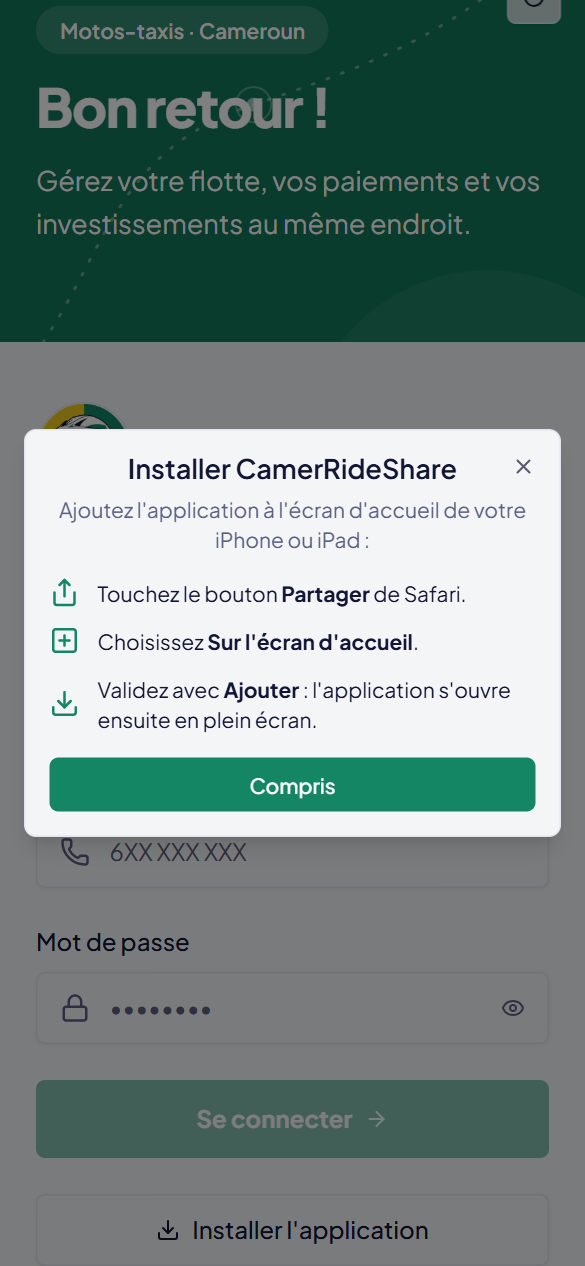
\includegraphics[height=0.42\textheight]{images/32-installation-iphone.png}}
\caption{Sur iPhone : la fenêtre d'explication.}\label{fig:iphone}
\end{figure}
\begin{enumerate}
  \item Ouvrez le logiciel dans \textbf{Safari}.
  \item Touchez le bouton \textbf{Partager} de Safari.
  \item Choisissez \bouton{Sur l'écran d'accueil}, puis \bouton{Ajouter}.
\end{enumerate}

\begin{astuce}
L'application installée \textbf{se met à jour toute seule} : à chaque nouvelle version, elle se renouvelle sans que vous ayez rien à faire. Si elle semble figée ou affiche un écran blanc, elle essaie de se réparer d'elle-même au bout de quelques secondes ; sinon, fermez-la complètement puis rouvrez-la.
\end{astuce}

% ═══ 3. TABLEAU DE BORD ══════════════════════════════════════════════════════
\section{Le tableau de bord}

C'est la page qui s'ouvre après la connexion. Elle répond à trois questions : \textit{combien ai-je investi, combien ai-je déjà reçu, et y a-t-il quelque chose à surveiller ?}

\capture{04-dashboard.png}{dashboard}{Le tableau de bord.}{0.6}
\begin{legende}
  \item[\mk{1}] \bouton{Télécharger Relevé PDF} : votre relevé officiel (voir ci-dessous).
  \item[\mk{2}] \textbf{Total investi} : le capital que vous avez apporté, avec le nombre de parts et de véhicules concernés. \bouton{Voir mon parc} ouvre la page correspondante.
  \item[\mk{3}] \textbf{Total récupéré} : ce que vous avez déjà perçu, et la proportion que cela représente du retour attendu.
  \item[\mk{4}] \textbf{Solde net} : ce que vous avez perçu, moins ce que vous avez investi. Le \textbf{ROI global} est ce solde rapporté au capital investi.
  \item[\mk{5}] \textbf{Reversement} : votre mode de versement (ici hebdomadaire), la date du prochain reversement, et la somme \textbf{à reverser maintenant}, c'est-à-dire ce que l'administrateur vous doit déjà.
  \item[\mk{6}] \textbf{À surveiller} : les véhicules qui peuvent retarder vos reversements.
  \item[\mk{7}] \textbf{Performance des revenus} : les sommes perçues, cumulées, sur la durée choisie avec les boutons \bouton{1 mois}, \bouton{3 mois}, \bouton{6 mois} et \bouton{1 an}.
  \item[\mk{8}] \textbf{Votre portefeuille de flotte} : un aperçu de vos véhicules. \bouton{Voir tout} ouvre la page \bouton{Mon parc}.
\end{legende}

\begin{retenir}
Un \textbf{solde net négatif} est normal au début : tant que vous n'avez pas reçu autant que ce que vous avez investi, il est négatif. Il remonte à chaque reversement. La mention rouge \textit{dont perte constatée} n'apparaît que lorsqu'un véhicule a été classé en perte ou qu'un contrat a pris fin sans que votre capital ait été entièrement récupéré.
\end{retenir}

\subsection{Télécharger votre relevé}

\capture{05-releve.png}{releve}{Le choix de la période du relevé.}{0.2}
\begin{enumerate}
  \item Cliquez sur \mk{1} \bouton{Télécharger Relevé PDF}.
  \item \mk{2} Choisissez la \textbf{période} : tout l'historique, ce mois-ci, le mois dernier, ce trimestre, cette année, l'année dernière ou une période personnalisée.
  \item \mk{3} Cliquez sur \bouton{Télécharger le PDF}.
\end{enumerate}

Le relevé est un document PDF prêt à être conservé ou imprimé. Le même bouton existe sur la page \bouton{Historique des revenus}.

\subsection{Les véhicules à surveiller}

Le bloc \bouton{À surveiller} liste les véhicules dont la situation peut retarder vos reversements :
\begin{itemize}
  \item \textbf{En panne} : le véhicule est immobilisé, il ne rapporte rien tant qu'il ne roule pas.
  \item \textbf{Retard} : le conducteur n'a pas versé tout ce qu'il devait (le nombre de semaines de retard et la somme restante sont indiqués).
  \item \textbf{Sans conducteur} : aucun revenu tant qu'un conducteur n'est pas affecté au véhicule.
\end{itemize}

Cliquez sur \bouton{Détails} pour ouvrir la fiche du véhicule.

\capture{06-surveiller.png}{surveiller}{La fiche d'un véhicule dont le conducteur est en retard.}{0.46}
\begin{legende}
  \item[\mk{1}] L'\textbf{avancement du remboursement} par le conducteur (ici semaine 20 sur 32, soit 63\,\%).
  \item[\mk{2}] L'\textbf{état des versements du conducteur} : à jour, en retard, sans conducteur\ldots Le retard est signalé à l'administrateur.
  \item[\mk{3}] \textbf{Investi ici} : votre apport sur ce véhicule. Les trois cartes voisines donnent ce que vous avez \textit{perçu}, ce que vous avez touché \textit{ce mois-ci} et ce que vous devriez toucher \textit{par semaine}.
  \item[\mk{4}] \textbf{Vos parts} : le détail de chaque part (voir \autoref{sec:parc}).
\end{legende}

\begin{astuce}
Un retard n'est pas une perte : l'administrateur relance le conducteur, et chaque semaine de retard \textit{prolonge} le calendrier de remboursement du conducteur. Mais vos reversements peuvent être décalés d'autant.
\end{astuce}

% ═══ 4. MON PARC ═════════════════════════════════════════════════════════════
\section{Mon parc : vos véhicules}\label{sec:parc}

La page \bouton{Mon parc} réunit tous les véhicules sur lesquels vous avez une part.

\capture{07-parc.png}{parc}{La page « Mon parc ».}{0.55}
\begin{legende}
  \item[\mk{1}] \textbf{Véhicules total} : le nombre de véhicules sur lesquels vous avez au moins une part. \mk{2} \textbf{En circulation} et \mk{3} \textbf{En maintenance} comptent ceux qui roulent et ceux qui sont en panne ou indisponibles. Ces trois cartes sont aussi des \textbf{boutons} : cliquez sur l'une d'elles pour filtrer la liste.
  \item[\mk{4}] Un \textbf{récapitulatif rapide} de vos véhicules, avec leur avancement.
  \item[\mk{5}] \textbf{Plus récents} : les parts prises ces 60 derniers jours.
  \item[\mk{6}] \textbf{Zone géographique} : filtrez par ville.
  \item[\mk{7}] La \textbf{recherche} : tapez une plaque d'immatriculation ou le nom d'un conducteur.
  \item[\mk{8}] Une \textbf{fiche de véhicule} : conducteur, plaque, statut (\textit{Actif}\ldots), avancement du remboursement, zone, nombre de parts, vos contrats, le total investi, le retour attendu, et votre \textbf{revenu du mois}. \bouton{Détails} ouvre la fiche complète.
\end{legende}

\subsection{Le détail d'un véhicule}

\capture{08-parc-detail-a.png}{detaila}{Haut de la fiche d'un véhicule.}{0.44}
\begin{legende}
  \item[\mk{1}] \textbf{Remboursement par le conducteur} : la semaine en cours sur la durée du contrat, le pourcentage, et la somme déjà versée sur la somme totale à rembourser.
  \item[\mk{2}] \textbf{État du conducteur} : à jour, en retard, sans conducteur, ou contrat terminé (dans ce dernier cas, la Société continue de vous verser votre part jusqu'au solde).
  \item[\mk{3}] \textbf{Investi ici} : votre capital sur ce véhicule, en une ou plusieurs parts.
  \item[\mk{4}] \textbf{Perçu} : ce que vous avez reçu, sur ce que vous devez recevoir au total.
  \item[\mk{5}] \textbf{Par semaine} : votre revenu hebdomadaire estimé, si le conducteur verse tout.
\end{legende}

\capture{08-parc-detail-b.png}{detailb}{Bas de la fiche d'un véhicule : vos parts et vos dernières sommes perçues.}{0.5}
\begin{legende}
  \item[\mk{6}] \textbf{Vos parts} : une ligne par apport.
  \item[\mk{7}] Pour chaque part : la \textbf{date et le montant de l'apport}, sa \textbf{part du prix d'achat}, ce qui a été \textbf{perçu} sur ce qui est \textbf{attendu}, et le \textbf{recouvrement}. Une mention indique si l'apport a été fait \textit{en cours de contrat} (voir \autoref{sec:marche}) et le rattrapage correspondant.
  \item[\mk{8}] \bouton{Contrat} : télécharge le contrat de cette part au format PDF (voir ci-dessous).
  \item[\mk{9}] \textbf{Dernières sommes perçues} : chaque versement, avec sa date, son montant et son état : \textit{À reverser} (l'administrateur ne vous l'a pas encore versé) ou \textit{Reversé le\ldots}
\end{legende}

\subsection{Vos contrats}

Chaque part est un contrat. Les boutons \bouton{Contrat $\cdot$ montant $\cdot$ date}, sur les fiches de véhicule, génèrent le \textbf{contrat PDF} de la part correspondante. Un message \bouton{Génération\ldots} s'affiche quelques secondes. Conservez ces documents : ils portent les informations de la société et les vôtres, qui doivent être justes (vérifiez votre profil dans les \hyperref[sec:parametres]{paramètres}).

% ═══ 5. MARCHÉ DES PARTS ═════════════════════════════════════════════════════
\section{Le marché des parts}\label{sec:marche}

La page \bouton{Marché des parts} présente les véhicules qui ont encore du capital à financer. Vous y proposez un apport ; \textbf{un administrateur valide chaque demande}.

\capture{09-marche.png}{marche}{La page « Marché des parts ».}{0.6}
\begin{legende}
  \item[\mk{1}] Le \textbf{rappel du risque} : lisez-le. Un investissement peut rapporter moins que prévu, ou ne pas être entièrement récupéré.
  \item[\mk{2}] La \textbf{recherche} : plaque, marque ou modèle.
  \item[\mk{3}] Le \textbf{tri} : \textit{Ajoutés récemment}, \textit{Plus de capital à financer} ou \textit{Plus avancés}.
  \item[\mk{4}] Les \textbf{zones} : filtrez par ville.
  \item[\mk{5}] Une \textbf{fiche de véhicule à financer} : le prix d'achat, le pourcentage déjà financé, la somme \textit{investissable}, un \textbf{exemple} chiffré pour 50\,000~XAF, et des étiquettes sur la situation du véhicule (\textit{Sans conducteur}, \textit{Nouveau véhicule}, \textit{Conducteur à jour} ou \textit{en retard}, ancienneté de service\ldots).
  \item[\mk{6}] \bouton{Investir dans ce véhicule}. Si vous avez déjà des parts sur ce véhicule, le bouton devient \bouton{Investir à nouveau} et la fiche rappelle ce que vous avez déjà investi.
  \item[\mk{7}] \textbf{Demande en attente} : votre demande est en cours d'examen. \bouton{Annuler} la retire tant qu'elle n'est pas traitée.
\end{legende}

\subsection{Faire une demande d'apport}

\capture{11-investir.png}{investir}{La fenêtre « Investir dans ce véhicule ».}{0.62}
\begin{enumerate}
  \item \mk{1} Saisissez le \textbf{montant de votre apport}, en francs CFA et sans espace. Il doit être d'au moins 50\,000~XAF et ne peut pas dépasser la somme encore investissable (affichée à droite des boutons).
  \item \mk{2} \bouton{Minimum} et \mk{3} \bouton{Maximum} remplissent le champ à votre place avec le plus petit ou le plus grand montant autorisé.
  \item \mk{4} Vérifiez le \textbf{récapitulatif} : le montant, la part du prix d'achat que cela représente, le \textbf{retour total} à 160\,\% et ce que vous recevrez \textbf{chaque semaine}.
  \item \mk{5} Cochez la case pour confirmer que vous avez \textbf{lu et compris le risque}. Sans cela, le bouton d'envoi reste grisé.
  \item \mk{6} Cliquez sur \bouton{Envoyer la demande}.
\end{enumerate}

Le logiciel vous avertit si le véhicule n'a pas de conducteur (il ne génère alors aucun revenu tant qu'il n'est pas réaffecté). Une demande est \textbf{sans engagement tant que l'administrateur ne l'a pas acceptée}.

\subsection{Investir dans un véhicule déjà en service}

Quand un véhicule a déjà reçu des versements, deux règles s'appliquent :
\begin{itemize}
  \item votre apport est \textbf{plafonné} : le retour de votre part ne peut pas dépasser \textbf{50\,\% de ce que le véhicule doit encore produire}. Le plafond est affiché dans la fenêtre, et la fiche du véhicule précise \textit{plafond du véhicule en cours de contrat} ;
  \item vous avez droit aux \textbf{semaines déjà écoulées} : c'est le \textbf{rattrapage}. Il est versé \textbf{en plus} de votre part habituelle, étalé sur 32 semaines à compter de la date de votre apport. Le montant du rattrapage et celui ajouté à chaque versement apparaissent dans le récapitulatif.
\end{itemize}

\subsection{Suivre vos demandes}

\capture{10-marche-demandes.png}{demandes}{Le suivi de vos demandes, en bas de la page.}{0.3}
\begin{legende}
  \item[\mk{1}] \textbf{Mes demandes} : toutes vos demandes de parts, avec la date et le montant.
  \item[\mk{2}] \textit{En attente} : l'administrateur ne s'est pas encore prononcé. \mk{3} \bouton{Annuler} retire la demande.
  \item[\mk{4}] \textit{Acceptée} : la part existe. \bouton{Voir dans Mon parc} ouvre le véhicule.
  \item[\mk{5}] \textit{Refusée} : le motif donné par l'administrateur est affiché sous la demande. \textit{Annulée} signifie que vous l'avez retirée vous-même.
\end{legende}

Vous êtes \textbf{toujours notifié} de la décision de l'administrateur (cloche), ainsi que de chaque nouvelle part enregistrée à votre nom.

% ═══ 6. HISTORIQUE DES REVENUS ═══════════════════════════════════════════════
\section{L'historique des revenus}

Cette page liste \textbf{toutes les sommes perçues} sur vos parts, versement après versement.

\capture{12-revenus.png}{revenus}{La page « Historique des revenus ».}{0.74}
\begin{legende}
  \item[\mk{1}] \bouton{Télécharger Relevé PDF} (voir \autoref{fig:releve}).
  \item[\mk{2}] \textbf{Revenu du mois}, avec l'évolution par rapport au mois précédent. \mk{3} \textbf{Dernier versement} : montant, véhicule et date. À droite, la \textbf{moyenne par véhicule} sur le mois.
  \item[\mk{4}] \textbf{Versement hebdomadaire} (ou mensuel, selon votre mode) : ce que vous avez \textit{déjà reçu}, ce qui est \textit{à recevoir (exigible)}, la \textit{période en cours} et la \textit{date du prochain versement}.
  \item[\mk{5}] La \textbf{recherche} : par nom de conducteur ou plaque. \mk{6} Le \textbf{filtre de statut} et \mk{7} le \textbf{filtre de période}.
  \item[\mk{8}] Le \textbf{statut} d'une somme : \textit{À recevoir} ou \textit{Versé le\ldots}
  \item[\mk{9}] \bouton{Voir le véhicule} ouvre la fiche du véhicule concerné.
\end{legende}

\subsection{Lire le tableau}

\begin{center}
\begin{tabularx}{\linewidth}{@{}L{3.6cm}X@{}}
\toprule
Date et heure & Le moment où la somme a été générée par un versement du conducteur.\\
Chauffeur & Le conducteur dont le versement est à l'origine de la somme. \textit{Grand Patron} désigne la Société elle-même : voir \textit{Échéance de la Société} ci-dessous.\\
Véhicule & La plaque du véhicule concerné.\\
Montant & Votre part de ce versement (en francs CFA).\\
Statut & \textit{À recevoir} : l'administrateur ne vous l'a pas encore reversée. \textit{Versé le\ldots} : vous l'avez reçue.\\
\bottomrule
\end{tabularx}
\end{center}

Deux étiquettes peuvent s'ajouter au statut :
\begin{itemize}
  \item \textbf{Échéance de la Société} : le conducteur a fini de rembourser son véhicule, mais votre part n'est pas encore entièrement payée. La Société continue alors de vous verser votre part jusqu'au solde.
  \item \textbf{dont rattrapage \ldots} : une partie de la somme correspond au rattrapage des semaines passées d'une part souscrite en cours de contrat.
\end{itemize}

\capture{13-revenus-statuts.png}{statuts}{Filtrer par statut.}{0.16}
Le filtre de statut propose \mk{1} \bouton{À recevoir} (ce que l'on ne vous a pas encore reversé) et \mk{2} \bouton{Déjà versées}. Le filtre de période propose tout l'historique, ce mois-ci, le mois dernier, ce trimestre, cette année, l'année dernière ou une période personnalisée. Les résultats s'affichent dix par dix : utilisez \bouton{Précédent} et \bouton{Suivant} en bas de la liste.

% ═══ 7. RAPPORTS ═════════════════════════════════════════════════════════════
\section{Les rapports et analyses}

La page \bouton{Rapports} analyse la performance de vos investissements sur la période de votre choix.

\capture{14-rapports-a.png}{rapportsa}{Haut de la page « Rapports ».}{0.7}
\begin{legende}
  \item[\mk{1}] \bouton{Télécharger le rapport (PDF)} : le rapport de la période choisie, en document.
  \item[\mk{2}] Le \textbf{filtre de période} : \bouton{Mois}, \bouton{Trimestre}, \bouton{Année}, \bouton{Tout}, ou \bouton{Personnalisé}. Les dates exactes sont rappelées sous les boutons.
  \item[\mk{3}] \textbf{Revenus de la période}, avec la comparaison à la période précédente.
  \item[\mk{4}] \textbf{ROI de la période} : les revenus de la période rapportés au capital investi.
  \item[\mk{5}] \textbf{Capital récupéré} : le pourcentage du retour attendu déjà perçu, avec les montants.
  \item[\mk{6}] \textbf{Solde net} : ce que vous avez perçu moins ce que vous avez investi.
  \item[\mk{7}] \textbf{Revenus perçus} : un graphique des sommes reçues, par semaine ou par mois selon la période. Le capital apporté pendant la période est rappelé dessous.
  \item[\mk{8}] \textbf{Prévisions du mois prochain} (voir ci-dessous).
\end{legende}

\subsection{Choisir une période personnalisée}

\capture{15-rapports-perso.png}{rapportsperso}{Le filtre de période personnalisée.}{0.2}
\begin{enumerate}
  \item Cliquez sur \mk{2} \bouton{Personnalisé} (les autres boutons, comme \mk{1} \bouton{Mois}, choisissent une période toute faite).
  \item Renseignez la date de début dans \mk{3} \bouton{Du} et la date de fin dans \mk{4} \bouton{Au}, avec le calendrier ou en tapant la date.
\end{enumerate}

\subsection{Les prévisions du mois prochain}

\capture{16-previsions.png}{previsions}{Les trois scénarios de prévision.}{0.35}
\begin{legende}
  \item[\mk{1}] \textbf{Contractuel} : les conducteurs versent chaque semaine l'intégralité de leur montant. C'est le scénario optimiste.
  \item[\mk{2}] \textbf{Rythme observé} : ce que vous avez réellement perçu sur les trois derniers mois complets.
  \item[\mk{3}] \textbf{Prudent} : 75\,\% du rythme observé.
  \item[\mk{4}] L'\textbf{estimation des revenus} du mois prochain pour le scénario choisi.
  \item[\mk{5}] Le \textbf{rendement sur 30 jours}, rapporté au capital engagé dans des véhicules actifs.
  \item[\mk{6}] Le délai \textbf{estimé} pour récupérer l'intégralité de votre capital, avec la somme qui reste à récupérer.
\end{legende}

\begin{attention}
Les prévisions sont des \textbf{estimations}, pas des garanties. Elles supposent que les conducteurs continuent de payer et que les véhicules continuent de rouler.
\end{attention}

\capture{14-rapports-b.png}{rapportsb}{Bas de la page « Rapports » : rentabilité et répartition.}{0.7}
\begin{legende}
  \item[\mk{9}] \textbf{Rentabilité par véhicule} : pour chaque véhicule, le capital investi, les revenus de la période, le ROI, le recouvrement et la \textbf{situation} : \textit{Performant}, \textit{À surveiller} (avec le nombre de semaines de retard), \textit{À l'arrêt} ou \textit{Contrat résilié}.
  \item[\mk{10}] \textbf{Répartition des revenus} : la part de chaque véhicule dans vos revenus de la période.
\end{legende}

% ═══ 8. PARAMÈTRES ═══════════════════════════════════════════════════════════
\section{Les paramètres}\label{sec:parametres}

La page \bouton{Paramètres} regroupe trois onglets. Les modifications ne sont \textbf{enregistrées} que lorsque vous cliquez sur \bouton{Enregistrer les modifications}, dans la barre du bas ; \bouton{Réinitialiser} annule ce que vous venez de saisir.

\subsection{Profil}

\capture{17-parametres-profil.png}{profil}{L'onglet « Profil ».}{0.5}
\begin{legende}
  \item[\mk{1}] Les trois onglets : \bouton{Profil}, \bouton{Notifications} et \bouton{Compte}.
  \item[\mk{2}] Votre \textbf{photo} : \bouton{Prendre une photo} utilise la caméra de l'appareil ; \bouton{importer une image} choisit un fichier.
  \item[\mk{3}] Votre \textbf{nom complet}, qui figure sur vos contrats et vos relevés.
  \item[\mk{4}] Votre \textbf{numéro de téléphone}, qui sert aussi d'\textbf{identifiant de connexion}.
  \item[\mk{5}] Votre \textbf{adresse e-mail} : elle reçoit votre rapport hebdomadaire et les messages de la plateforme.
  \item[\mk{6}] \bouton{Modifier} permet de changer votre mot de passe. Pour votre sécurité, le mot de passe n'est jamais affiché.
  \item[\mk{7}] \bouton{Enregistrer les modifications}.
\end{legende}

\begin{astuce}
Choisissez un mot de passe que vous n'utilisez nulle part ailleurs, et changez celui qui vous a été communiqué à la création de votre compte.
\end{astuce}

\subsection{Notifications}\label{sec:notifs}

\capture{18-parametres-notifications.png}{notifs}{L'onglet « Notifications ».}{0.4}
\begin{legende}
  \item[\mk{1}] \textbf{Rapport hebdomadaire par e-mail} : chaque lundi matin, vos revenus de la semaine écoulée, le capital récupéré et les véhicules à surveiller.
  \item[\mk{2}] \textbf{Revenus et reversements} : une notification à chaque versement du conducteur qui vous est reversé, à chaque reversement de l'administrateur et à chaque changement de mode de versement.
  \item[\mk{3}] \textbf{État des véhicules} : une notification quand l'un de vos véhicules tombe en panne, devient indisponible, reprend la route ou est entièrement payé.
  \item[\mk{4}] Certaines notifications sont \textbf{toujours envoyées}, car elles engagent votre capital : décisions sur vos demandes de parts, nouvelles parts, résiliations de contrat.
  \item[\mk{5}] \bouton{Envoyer le rapport maintenant} : vous envoie le rapport à votre adresse e-mail sans attendre le lundi.
\end{legende}

\subsection{Compte}

\capture{19-parametres-compte.png}{compte}{L'onglet « Compte ».}{0.45}
\begin{legende}
  \item[\mk{1}] Les informations de votre compte, \textbf{en lecture seule} : la date d'inscription, le nombre de parts ouvertes et de véhicules, et votre \textbf{mode de versement}. Ce mode (\textit{Hebdomadaire} ou \textit{Mensuel}) est fixé par l'administrateur ; contactez-le pour le changer.
  \item[\mk{2}] \textbf{Thème sombre} : réglage propre à cet appareil.
  \item[\mk{3}] \bouton{Déconnexion}.
\end{legende}

% ═══ 9. QUAND SUIS-JE PAYÉ ═══════════════════════════════════════════════════
\section{Quand et comment suis-je payé ?}

\subsection{Le calendrier des reversements}

\begin{center}
\begin{tabularx}{\linewidth}{@{}L{3.6cm}X@{}}
\toprule
Mode hebdomadaire & L'administrateur vous reverse vos gains \textbf{chaque lundi}, pour la semaine écoulée.\\
Mode mensuel & L'administrateur vous reverse vos gains \textbf{le premier de chaque mois}, pour le mois écoulé.\\
Période en cours & Ce que vous avez déjà gagné sur la période qui n'est pas terminée. Ce n'est pas encore exigible, mais l'administrateur peut vous le verser à l'avance.\\
\bottomrule
\end{tabularx}
\end{center}

La page \bouton{Historique des revenus} vous donne à tout moment la \textbf{date du prochain versement} et la somme \textbf{déjà exigible}. Chaque reversement fait l'objet d'une notification et passe dans l'état \textit{Versé le\ldots}

\subsection{Ce qui peut retarder vos reversements}

\begin{center}
\begin{tabularx}{\linewidth}{@{}L{3.6cm}X@{}}
\toprule
Conducteur en retard & Il n'a pas versé tout ce qu'il devait cette semaine. Chaque semaine de retard prolonge son calendrier. L'administrateur le relance.\\
Véhicule en panne & Il ne roule pas, donc il ne génère pas de versement.\\
Sans conducteur & Aucun revenu tant qu'un conducteur n'est pas affecté. L'administrateur peut le réaffecter.\\
Contrat résilié & Le contrat du conducteur ou le vôtre a pris fin : vous êtes informé par notification, avec le détail de ce que vous avez perçu et de ce qui vous est remboursé ou réaffecté.\\
\bottomrule
\end{tabularx}
\end{center}

\begin{retenir}
Si un contrat prend fin avant que votre capital soit entièrement récupéré, l'administrateur décide, au cas par cas, de vous \textbf{rembourser} une partie de ce capital et/ou de le \textbf{réaffecter} à un autre véhicule. Les sommes que vous avez déjà perçues \textbf{vous restent acquises}. Vous êtes prévenu de chaque décision.
\end{retenir}

% ═══ 10. ROUTINE ═════════════════════════════════════════════════════════════
\section{Votre routine d'investisseur}

\subsection{Chaque semaine}
\begin{enumerate}
  \item Ouvrez le \textbf{tableau de bord} : regardez le solde net, la somme exigible et les véhicules à surveiller.
  \item Lisez vos \textbf{notifications} (la cloche) et votre \textbf{rapport hebdomadaire} reçu le lundi par e-mail.
  \item Après un reversement, vérifiez dans \bouton{Historique des revenus} que la somme est bien passée à l'état \textit{Versé le\ldots}
\end{enumerate}

\subsection{Chaque mois}
\begin{enumerate}
  \item Consultez la page \bouton{Rapports} sur la période \bouton{Mois} : revenus, ROI et rentabilité de chaque véhicule.
  \item Téléchargez votre \textbf{relevé} pour vos archives.
  \item Regardez le \bouton{Marché des parts} si vous souhaitez réinvestir.
\end{enumerate}

\subsection{Bonnes pratiques}
\begin{itemize}
  \item \textbf{Ne partagez jamais} votre mot de passe, et déconnectez-vous d'un ordinateur partagé.
  \item Gardez votre \textbf{adresse e-mail à jour} : c'est là que vous recevez votre rapport hebdomadaire et les messages importants.
  \item \textbf{Conservez vos contrats PDF} et vos relevés.
  \item Ne comptez jamais sur le retour de 160\,\% comme sur une certitude : \textbf{diversifiez} vos apports entre plusieurs véhicules.
\end{itemize}

% ═══ 11. DÉPANNAGE ═══════════════════════════════════════════════════════════
\section{Que faire si\ldots}

\begin{center}
\begin{tabularx}{\linewidth}{@{}>{\bfseries\raggedright}p{4.4cm}X@{}}
\toprule
Je n'arrive pas à me connecter & Vérifiez le numéro (sans espaces) et le mot de passe. Après plusieurs essais ratés, attendez quelques minutes. Si vous avez oublié votre mot de passe, contactez l'administrateur : il peut le réinitialiser.\\
\midrule
Je n'ai pas reçu un reversement & Regardez dans \bouton{Historique des revenus} avec le filtre \textit{À recevoir} : la somme est peut-être déjà exigible mais pas encore versée. Regardez aussi si le conducteur est en retard ou si le véhicule est en panne (tableau de bord, \bouton{À surveiller}). Sinon, contactez l'administrateur.\\
\midrule
Un véhicule est « à surveiller » & Ouvrez sa fiche pour connaître la cause : panne, retard du conducteur ou absence de conducteur. L'administrateur est déjà informé des retards.\\
\midrule
Ma demande de part est restée « en attente » & L'administrateur doit la valider. Vous pouvez l'annuler à tout moment tant qu'elle n'est pas traitée (\bouton{Marché des parts}, \bouton{Mes demandes}).\\
\midrule
Je ne peux pas investir autant que je le souhaite & Le montant maximum est celui qui reste à financer sur le véhicule. Sur un véhicule déjà en service, il est aussi plafonné à 50\,\% de ce que le véhicule doit encore produire.\\
\midrule
Je veux changer de mode de versement & Contactez l'administrateur : le mode (hebdomadaire ou mensuel) est fixé de son côté.\\
\midrule
Je ne reçois pas les e-mails & Vérifiez l'adresse e-mail de votre profil et regardez dans vos courriers indésirables. Vérifiez aussi que le rapport hebdomadaire est activé dans \bouton{Paramètres}, onglet \bouton{Notifications}.\\
\midrule
Le logiciel affiche une erreur ou reste bloqué & Actualisez la page. Sur l'application installée, fermez-la complètement puis rouvrez-la : elle se met à jour et se répare seule. Une bannière vous prévient aussi si votre connexion Internet est coupée.\\
\bottomrule
\end{tabularx}
\end{center}

% ═══ INDEX DES TÂCHES ════════════════════════════════════════════════════════
\section{Index des tâches courantes}\label{sec:taches}

\begin{center}
\begin{tabularx}{\linewidth}{@{}Xr@{}}
\toprule
\textbf{Je veux\ldots} & \textbf{Page}\\
\midrule
me connecter, installer l'application & \pageref{fig:connexion}\\
comprendre mon solde net et mon ROI & \pageref{fig:dashboard}\\
télécharger mon relevé PDF & \pageref{fig:releve}\\
voir les véhicules qui peuvent retarder mes reversements & \pageref{fig:surveiller}\\
voir tous mes véhicules & \pageref{fig:parc}\\
voir le détail d'une part, télécharger un contrat & \pageref{fig:detailb}\\
trouver un véhicule dans lequel investir & \pageref{fig:marche}\\
faire une demande d'apport & \pageref{fig:investir}\\
suivre ou annuler une demande & \pageref{fig:demandes}\\
voir ce que j'ai reçu et ce qui reste à recevoir & \pageref{fig:revenus}\\
analyser mes performances par véhicule & \pageref{fig:rapportsb}\\
estimer mes revenus du mois prochain & \pageref{fig:previsions}\\
changer mon mot de passe ou ma photo & \pageref{fig:profil}\\
choisir mes notifications & \pageref{fig:notifs}\\
connaître mon mode de versement & \pageref{fig:compte}\\
\bottomrule
\end{tabularx}
\end{center}

\vfill
\begin{center}\small\color{gris}
Guide rédigé par Abdoulrahim Momo Aboubakar -- CamerRideShare, novembre 2026.\\
Les captures d'écran présentent des données fictives de démonstration.
\end{center}

\end{document}
